% ============================================================
% BEAMER SCRIPT: Duality Gap in Dual Convex Optimization of ReLU Neural Networks
% Phase P8 — Oral Presentation Branch
% Duration: 8 minutes | Audience: mixed_academic | Goal: survey
% Venue: conference_talk | Q&A: after_only
% Emphasis: Pilanci & Ergen (Stanford)
%
% HOW TO USE THIS FILE:
%   1. Replace [Abhinav Mallick] and [Sri Venkateswara College] in the title block.
%   2. Replace PLACEHOLDER figure environments with actual TikZ drawings
%      or external PDF/PNG files (descriptions are in the % comments).
%   3. Speaking notes appear as % SPEAKING NOTES: comments immediately
%      above each \begin{frame}.
%   4. Compile with: tectonic beamer-script.tex
%      (or: pdflatex beamer-script.tex  run twice)
%
% TIMING OVERVIEW:
%   Act 1 (Motivation):      1:30  — Slides 1–2
%   Act 2 (Background):      2:30  — Slides 3–4
%   Act 3 (Core Results):    3:00  — Slides 5–6
%   Act 4 (Close):           1:00  — Slides 7–8
%   Appendix (Q&A backups):  —     — B1–B4
% ============================================================

\documentclass[aspectratio=169]{beamer}

% ============================================================
% PREAMBLE
% ============================================================
\usepackage{amsmath, amssymb, amsthm}
\usepackage{mathtools}
\usepackage{bm}
\usepackage{graphicx}
\usepackage{booktabs}
\usepackage{hyperref}
\usepackage{tikz}
\usetikzlibrary{positioning}
\usepackage{xcolor}
\usepackage[backend=bibtex, style=authoryear, maxcitenames=2, maxbibnames=99]{biblatex}
\addbibresource{references.bib}

% --- Theme (speaker may change) ---
\usetheme{Madrid}
\usecolortheme{default}
\setbeamertemplate{navigation symbols}{}

% Reduce bibliography font size to fit on a slide
\renewcommand*{\bibfont}{\tiny}

% ============================================================
% NOTATION MACROS (from Section 1, knowledge-base.md)
% ============================================================
% Training problem dimensions
\newcommand{\nn}{n}                          % number of training samples
\newcommand{\dd}{d}                          % input feature dimension
\newcommand{\mm}{m}                          % network width (hidden neurons)
\newcommand{\LL}{L}                          % network depth
\newcommand{\KK}{K}                          % number of parallel branches

% Data
\newcommand{\Xmat}{\mathbf{X}}              % data matrix, n x d
\newcommand{\yvec}{\mathbf{y}}              % label vector, n x 1
\newcommand{\uvec}{\mathbf{u}}              % hidden-layer weight vector

% Network notation
\newcommand{\relu}[1]{(#1)_+}              % ReLU activation: (t)_+
\newcommand{\alphaj}{\alpha_j}             % scalar output-layer weight
\newcommand{\betareg}{\beta}               % weight-decay regularization strength

% Duality
\newcommand{\Pstar}{P^*}                   % primal optimal value
\newcommand{\Dstar}{D^*}                   % dual optimal value
\newcommand{\gap}{\text{gap}}              % duality gap = P* - D*
\newcommand{\mstar}{m^*}                   % critical network width

% Activation patterns
\newcommand{\Di}{D_i}                      % diagonal ReLU activation pattern matrix
\newcommand{\PP}{P}                        % number of distinct hyperplane arrangement patterns
\newcommand{\rrank}{r}                     % rank of data matrix X

% Approximation
\newcommand{\ptildestar}{\tilde{p}^*}      % optimal value of O(log n)-pattern relaxation
\newcommand{\CC}{C}                        % universal constant in Kim-Pilanci bound

% Norms
\newcommand{\nucnorm}[1]{\|#1\|_{*}}       % nuclear norm (sum of singular values)
\newcommand{\schattennorm}[1]{\|#1\|_{S_{2/L}}}  % Schatten-2/L quasi-norm

% ============================================================
% TITLE INFORMATION — FILL IN BEFORE PRESENTING
% ============================================================
\title[Convex ReLU Networks]{%
  Duality Gap in Dual Convex Optimization of ReLU Networks\\[4pt]%
}
% \subtitle{A survey, 2020--2025 \quad (Emphasis: Pilanci \& Ergen)}
\author[Abhinav Mallick]{Abhinav Mallick\\[2pt]\normalsize (1722043)\\[8pt]
\small Department of Mathematics, Sri Venkateswara College, University of Delhi\\[6pt]
Supervisor: Ms.\ Pratibha Gaur}
\institute[]{}
\date{April 9, 2026\\[4pt]{\normalsize Presented at}\\[2pt]{\normalsize SVC-SPARK Multidisciplinary International Conference 2026}}

% ============================================================
\begin{document}
% ============================================================

% ============================================================
% ACT 1: MOTIVATION (target: 1:30, Slides 1-2)
% ============================================================

% ---- SLIDE 1: TITLE (0:00-0:15, 15 seconds) ----
% SPEAKING TIME: ~15 seconds
% TIMING CHECK: End of Act 1 is 1:30. Slide 1 eats only 15 sec.
%
% SPEAKING NOTES:
% Say nothing during Slide 1. Let the title register for 3-4 seconds.
% Then begin the bridge line to Slide 2 immediately:
% "For the last ten years we have told students that neural network
%  training is non-convex, and that SGD has no right to work.
%  Here is the question this talk is going to answer."
% (The bridge line belongs spoken over the transition, not over the title.)
%
% IF RUNNING LONG: Cut the silence period; go straight to the bridge line.
%
\begin{frame}
  \titlepage
  % Small acknowledgement line at the foot (uncomment and edit):
  % \vfill
  % \tiny Work of M.\ Pilanci, T.\ Ergen, and collaborators -- Stanford University.
\end{frame}


% ---- SLIDE 2: THE MYSTERY (0:15-1:30, 75 seconds) ----
% SPEAKING TIME: ~75 seconds (longest single slide; if rushing, you are on track)
% TIMING CHECK: End of Slide 2 = 1:30 = end of Act 1.
%
% SPEAKING NOTES:
% Open with the motivator open question (OQ2):
% "Stochastic gradient descent was designed for convex problems. We run it on
%  objectives that are provably non-convex -- loss surfaces studded with local
%  minima and saddle points -- and despite a decade of optimization theory
%  telling us this should not work, we get models that generalize.
%  The folk explanation is overparameterization plus good initialization plus
%  some luck. I want to argue today that this explanation is incomplete, and
%  that a much more satisfying answer exists."
% [Pause.]
% "The answer is that the problem was secretly convex all along. And the bridge
%  between the non-convex thing you trained and the convex thing you could have
%  solved is called strong duality."
%
% BRIDGE TO SLIDE 3:
% "To explain what that means I need to define one object -- the duality gap
%  -- and then I can state the result that started this programme."
%
% IF RUNNING LONG: Drop bullet 4 (folk answer); speak it instead of showing it.
%
\begin{frame}{Motivation: Why Does SGD Work?}
  \begin{columns}[c]
    \begin{column}{0.5\textwidth}
      \begin{itemize}
        \item SGD was designed for convex problems
        \item We run it on provably non-convex losses
        \item It works anyway --- why?
        \item Common explanation: overparameterization and favourable initialisation
        \item \textbf{A more precise answer emerged in 2020}
      \end{itemize}
    \end{column}
    \begin{column}{0.48\textwidth}
      \begin{center}
        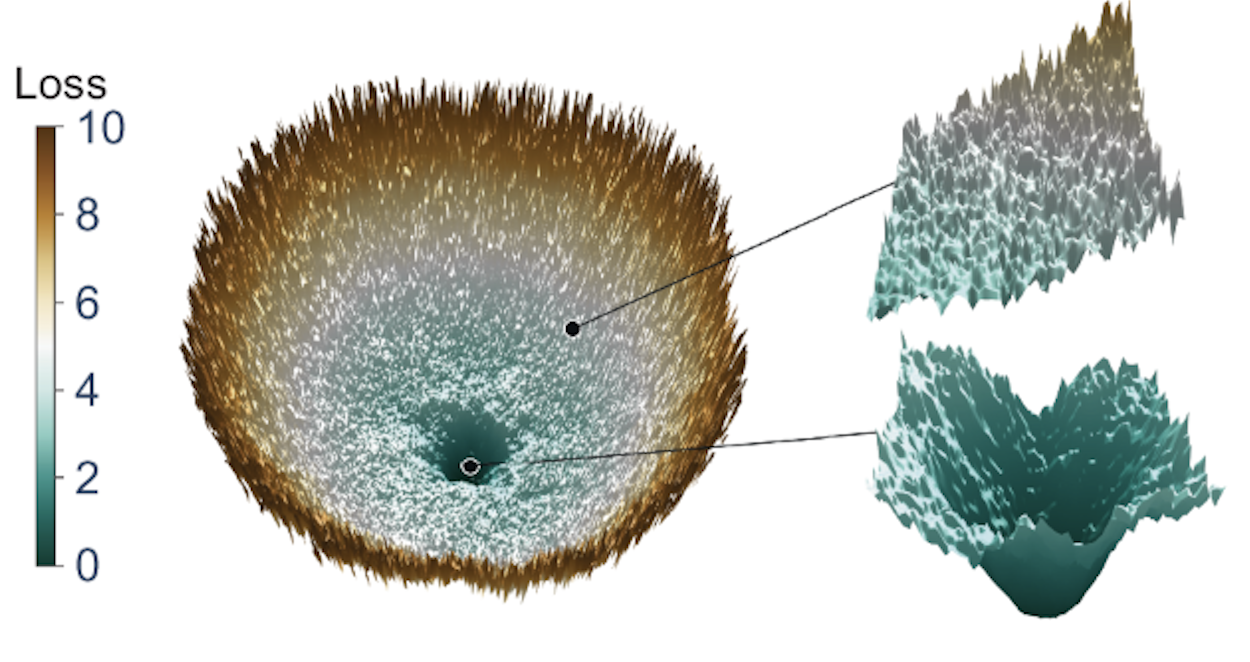
\includegraphics[width=\textwidth,height=0.48\textheight,keepaspectratio]{loss-landscape.png}
      \end{center}
    \end{column}
  \end{columns}
  % Source: Wang, Ergen & Pilanci 2021 (arxiv-2110.06482) frame the open
  % problem at line 22: "underlying theoretical reasons for this remains
  % an open problem."
\end{frame}


% ============================================================
% ACT 2: BACKGROUND --- BUILDING THE BRIDGE (target: 2:30, Slides 3-4)
% ============================================================

% ---- SLIDE 3: DUALITY GAP IN 45 SECONDS (1:30-2:15, 45 seconds) ----
% SPEAKING TIME: ~45 seconds (shortest content slide --- do not linger)
% TIMING CHECK: End of Slide 3 = 2:15.
%
% SPEAKING NOTES:
% "Every optimization problem -- what we call the 'primal' -- has a companion
%  problem, called its 'dual,' whose optimal value is always a lower bound on
%  the original. This is weak duality, and it is always true, even for
%  non-convex problems. The gap is the difference between the two: how much
%  the dual underestimates the primal. For convex problems -- least squares,
%  Lasso, linear programming -- the gap is zero: the dual and primal touch.
%  For non-convex problems -- almost everything in neural networks -- the gap
%  is usually strictly positive. The reason this talk exists is that for a
%  specific family of non-convex problems, namely ReLU networks with weight
%  decay, the gap is also zero. That is the result I want to show you first."
%
% BRIDGE TO SLIDE 4: "That surprising fact is the result from 2020."
%
% WARNING: Do not overexplain this slide. It is vocabulary, not content.
% One minute maximum. If a listener looks confused, Slide 4 demonstrates it.
%
% IF RUNNING LONG: Collapse into Slide 4 -- spend 15 sec defining P* >= D*
% inline at the top of Slide 4. Saves 30 seconds. Cost: cognitive load during climax.
%
\begin{frame}{Duality Gap: Key Definitions}
  \begin{center}
    \vspace{0.4em}
    {\large Every optimization problem has a companion \textbf{dual}.}\\[1.2em]
    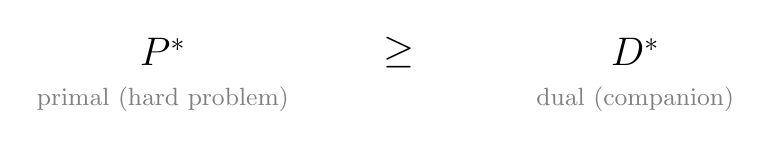
\begin{tikzpicture}
      \node[font=\Large] (primal) at (-3,0) {$\Pstar$};
      \node[font=\Large] at (0,0)   {$\geq$};
      \node[font=\Large] (dual)   at (3,0)  {$\Dstar$};
      \node[font=\small, gray] at (-3,-0.6) {primal (hard problem)};
      \node[font=\small, gray] at  (3,-0.6) {dual (companion)};
    \end{tikzpicture}\\[1em]
    $\gap = \Pstar - \Dstar$\\[0.5em]
    $\textbf{strong duality} \iff \gap = 0$\\[1.2em]
    \textit{\small For convex problems the gap is zero.\ For non-convex --- usually not.}
  \end{center}
  \begin{block}{}
    \centering
    For ReLU networks with weight decay, the gap turns out to be zero.
  \end{block}
\end{frame}


% ---- SLIDE 4: THE BRIDGE IS BUILT --- PILANCI & ERGEN 2020 (2:15-4:00, 105 sec) ----
% SPEAKING TIME: ~105 seconds = 1:45 (the only slide with an equation on screen)
% TIMING CHECK: End of Slide 4 = 4:00 = end of Act 2.
%
% SPEAKING NOTES:
% Plain language first:
% "For a two-layer ReLU network with ordinary weight decay -- nothing fancy,
%  no architectural tricks -- the non-convex training loss has a finite-
%  dimensional convex reformulation. The two programs have the same optimal
%  value. The duality gap is zero."
%
% Walk through the equation (do not read symbols aloud --- describe terms):
% "The first term is the training loss. The second term is weight decay.
%  The sum is over the m hidden neurons. And (dot)_+ is the ReLU."
%
% State the width caveat:
% "Width m has to be at least some critical value m*. That m* is bounded
%  by n+1 -- if the network is wider than roughly the number of training
%  points you are guaranteed zero gap."
%
% State the implication:
% "The 'non-convex' problem you were solving with SGD is, globally, a
%  second-order cone program you could hand to any convex solver.
%  That is a sentence the textbooks do not tell you."
%
% Plant the IOU (repaid on Slide 6):
% "The convex program has (n/r)^r variables -- polynomial in n, exponential
%  in data rank. Clean theoretically, not yet practical. Hold that thought;
%  we will come back to it."
%
% BRIDGE TO SLIDE 5: "Two layers are secretly convex. What happens when
% you go deeper?"
%
% IF RUNNING LONG: Cut the complexity objection sentence; it can be absorbed
% into Slide 6 without loss.
%
\begin{frame}{Convex Reformulation: Pilanci \& Ergen (2020)}

  \textbf{Non-convex primal:}
  \vspace{-0.5em}
  \[
    \min_{\{\uvec_j,\,\alphaj\}_{j=1}^{\mm}}
    \frac{1}{2} \left\|
      \sum_{j=1}^{\mm} \relu{\Xmat \uvec_j} \alphaj - \yvec
    \right\|_2^2
    + \frac{\betareg}{2} \sum_{j=1}^{\mm}
      \left( \|\uvec_j\|_2^2 + \alphaj^2 \right)
    \tag{primal}
  \]

  \vspace{-0.3em}
  \begin{center}
    \large$\Downarrow$\quad \textbf{zero duality gap}
  \end{center}
  \vspace{-0.5em}

  \textbf{Equivalent convex program (SOCP):}
  \begin{itemize}
    \item $O\!\left((\nn/\rrank)^{\rrank}\right)$ variables; finite, exact
    \item Width condition: $\mm \geq \mstar \leq \nn+1$
  \end{itemize}

  \vspace{0.3em}
  \begin{alertblock}{Theorem 1 \normalfont\small[Pilanci \& Ergen, 2020]}
    Two-layer ReLU $+$ weight decay admits an exact convex reformulation.
    Strong duality holds for $\mm \geq \mstar$.
  \end{alertblock}

  % SOURCE: Pilanci & Ergen 2020, arxiv-2002.10553, Theorem 1 (lines 155-162)
  % and Remark 3.2 (line 172) for the complexity bound.
  % Equation labels match paper eqns (2) and (8).
\end{frame}


% ---- SLIDE 4b: ARCHITECTURE VARIABLES --- VISUAL COMPANION ----
% SPEAKING NOTES:
% "Let me make those variables concrete. The network has d-dimensional input,
%  m hidden neurons, and one output. Weight vectors u_j feed the input into
%  neuron j; after ReLU we scale by alpha_j to get the output. The diagonal
%  matrix D_i encodes which neurons fire for training sample i -- the
%  hyperplane arrangement pattern. These D_i are what drive both the exact
%  convex reformulation and the complexity count (n/r)^r."
%
\begin{frame}{Architecture of the Primal Two-Layer ReLU Network}
  \begin{center}
  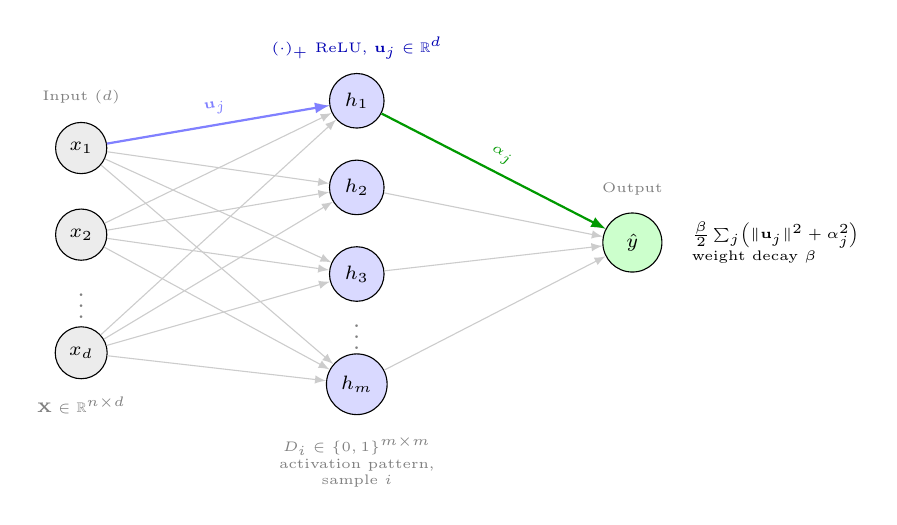
\begin{tikzpicture}[
      neuron/.style={circle, draw, minimum size=0.62cm, font=\scriptsize},
      >=latex
  ]
    % --- Input layer (3 visible nodes representing d inputs) ---
    \node[neuron, fill=gray!15] (in1) at (0, 2.2)  {$x_1$};
    \node[neuron, fill=gray!15] (in2) at (0, 1.1)  {$x_2$};
    \node[font=\small, gray]    (dots1) at (0, 0.3)  {$\vdots$};
    \node[neuron, fill=gray!15] (in3) at (0, -0.4) {$x_d$};
    \node[font=\tiny, gray, below=0.1cm of in3] {$\mathbf{X}\in\mathbb{R}^{n\times d}$};
    \node[font=\tiny, gray, above=0.1cm of in1] {Input ($d$)};

    % --- Hidden layer (4 visible nodes representing m neurons) ---
    \node[neuron, fill=blue!15] (h1) at (3.5, 2.8)  {$h_1$};
    \node[neuron, fill=blue!15] (h2) at (3.5, 1.7)  {$h_2$};
    \node[neuron, fill=blue!15] (h3) at (3.5, 0.6)  {$h_3$};
    \node[font=\small, gray]    (dots2) at (3.5, -0.1) {$\vdots$};
    \node[neuron, fill=blue!15] (h4) at (3.5, -0.8) {$h_m$};
    \node[font=\tiny, blue!70!black, above=0.05cm of h1]
      {$(\cdot)_+$ ReLU, $\mathbf{u}_j\in\mathbb{R}^d$};
    \node[font=\tiny, gray, align=center, below=0.15cm of h4]
      {$D_i\in\{0,1\}^{m\times m}$\\activation pattern,\\ sample $i$};

    % --- Output layer ---
    \node[neuron, fill=green!20, minimum size=0.75cm] (out) at (7, 1.0) {$\hat{y}$};
    \node[font=\tiny, gray, above=0.1cm of out] {Output};
    \node[font=\tiny, align=left, right=0.25cm of out]
      {$\frac{\beta}{2}\sum_j\!\left(\|\mathbf{u}_j\|^2+\alpha_j^2\right)$\\weight decay $\beta$};

    % --- Edges input -> hidden (u_j label on one representative edge) ---
    \foreach \src in {in1,in2,in3} {
      \foreach \dst in {h1,h2,h3,h4} {
        \draw[->, gray!40, thin] (\src) -- (\dst);
      }
    }
    \draw[->, blue!50, thick] (in1) -- (h1)
      node[midway, above, font=\tiny, sloped] {$\mathbf{u}_j$};

    % --- Edges hidden -> output (alpha_j label on one representative edge) ---
    \foreach \src in {h1,h2,h3,h4} {
      \draw[->, gray!40, thin] (\src) -- (out);
    }
    \draw[->, green!60!black, thick] (h1) -- (out)
      node[midway, above, font=\tiny, sloped] {$\alpha_j$};

  \end{tikzpicture}
  \end{center}

  \vspace{-0.3em}
  \begin{center}
    \tiny Two-layer ReLU network: $m$ hidden neurons, $n$ training samples,
    $P = O((n/r)^r)$ distinct activation patterns $D_i$.
  \end{center}
\end{frame}


% ============================================================
% ACT 3: CORE RESULTS --- CLIMAX AND RECOVERY (target: 3:00, Slides 5-6)
% ============================================================

% ---- SLIDE 5: THE CLIMAX --- DEPTH BREAKS, PARALLELISM RESTORES (4:00-5:45, 105 sec) ----
% SPEAKING TIME: ~105 seconds = 1:45  --- THE OVER-INVESTED SLIDE
% TIMING CHECK: Climax at 4:52 midpoint = ~61% of 8 min (appropriate for short talk).
%
% SPEAKING NOTES:
% Set the expectation:
% "You might expect the duality gap to grow smoothly with depth -- deeper
%  networks are 'more non-convex,' so the gap should get worse the further
%  you go."
%
% Reveal the actual result:
% "That is not what happens. At L=2 the gap is exactly zero. At L=3, for a
%  standard deep network with vector output, the gap *jumps* to something
%  strictly positive. Wang, Ergen, and Pilanci compute it in closed form --
%  it is a gap between a Schatten quasi-norm and the nuclear norm, and it is
%  zero only when all singular values of your label matrix are equal."
%
% [PAUSE -- let it land. The pause should feel slightly uncomfortable.]
%
% Deliver the twist:
% "But -- and this is the beautiful part -- if you rearrange exactly the same
%  network as K independent parallel branches that sum at the output, the gap
%  snaps back to zero at any depth."
%
% Disambiguation (first use of 'parallel'):
% "By parallel I mean architecturally parallel -- not GPU parallelism."
%
% Connect to practice:
% "And now look at what modern architectures actually do. Inception, ResNeXt,
%  ResNets with weight decay -- these already have parallel branch structure.
%  The paper suggests this may be part of why they train more reliably.
%  Architecture, not depth, is the villain."
%
% BRIDGE TO SLIDE 6:
% "So the bridge holds for two-layer networks, and for parallel networks of
%  any depth -- but the convex program still has that (n/r)^r variables
%  problem. Can any of this actually run on real data?"
%
% IF RUNNING LONG: Cut the "modern architectures" connection; state it in one
% sentence during the bridge to Slide 6.
%
\begin{frame}{Depth vs.\ Architecture: Effect on the Duality Gap}

  \begin{columns}[c]
    \begin{column}{0.44\textwidth}
      \begin{block}{\textcolor{red}{Standard $\LL$-layer network}}
        \begin{center}
          % FIGURE DESCRIPTION: Sequential L-layer network as column of boxes:
          % Input -> Layer 1 -> Layer 2 -> Layer 3 -> Output.
          % TO REPLACE: draw in TikZ or use figures/slide5_sequential.pdf
          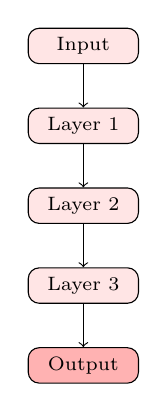
\begin{tikzpicture}[node distance=0.55cm, every node/.style={
              draw, rounded corners, minimum width=1.4cm, minimum height=0.4cm,
              font=\scriptsize, fill=red!10}]
            \node (inp) {Input};
            \node (l1) [below=of inp] {Layer 1};
            \node (l2) [below=of l1]  {Layer 2};
            \node (l3) [below=of l2]  {Layer 3};
            \node (out) [below=of l3, fill=red!30] {Output};
            \draw[->] (inp)--(l1); \draw[->] (l1)--(l2);
            \draw[->] (l2)--(l3); \draw[->] (l3)--(out);
          \end{tikzpicture}
        \end{center}
        \centering
        \textcolor{red}{$\Pstar > \Dstar$ for $\LL \geq 3$}
      \end{block}
    \end{column}
    \hfill
    \begin{column}{0.52\textwidth}
      \begin{block}{\textcolor{green!60!black}{Parallel ($\KK$ branches) network}}
        \begin{center}
          % FIGURE DESCRIPTION: K=4 parallel branches, each an L-layer path,
          % outputs summed at a plus node.
          % TO REPLACE: draw in TikZ or use figures/slide5_parallel.pdf
          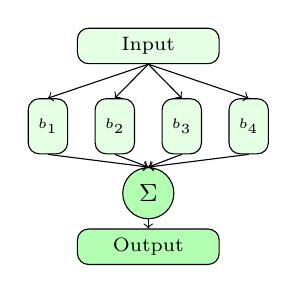
\begin{tikzpicture}[scale=0.85]
            % Input node at top
            \node[draw, rounded corners, fill=green!10, font=\scriptsize,
                  minimum width=1.8cm] (inp) at (0,2) {Input};
            % Four branch nodes
            \node[draw, rounded corners, fill=green!10, font=\tiny,
                  minimum width=0.5cm, minimum height=0.7cm] (b1) at (-1.5,0.8) {$b_1$};
            \node[draw, rounded corners, fill=green!10, font=\tiny,
                  minimum width=0.5cm, minimum height=0.7cm] (b2) at (-0.5,0.8) {$b_2$};
            \node[draw, rounded corners, fill=green!10, font=\tiny,
                  minimum width=0.5cm, minimum height=0.7cm] (b3) at (0.5,0.8)  {$b_3$};
            \node[draw, rounded corners, fill=green!10, font=\tiny,
                  minimum width=0.5cm, minimum height=0.7cm] (b4) at (1.5,0.8)  {$b_4$};
            % Sum node
            \node[draw, circle, fill=green!30, font=\small] (sum) at (0,-0.2) {$\Sigma$};
            % Output node
            \node[draw, rounded corners, fill=green!30, font=\scriptsize,
                  minimum width=1.8cm] (out) at (0,-1.0) {Output};
            % Arrows from input to branches
            \draw[->] (inp.south) -- (b1.north);
            \draw[->] (inp.south) -- (b2.north);
            \draw[->] (inp.south) -- (b3.north);
            \draw[->] (inp.south) -- (b4.north);
            % Arrows from branches to sum
            \draw[->] (b1.south) -- (sum.north);
            \draw[->] (b2.south) -- (sum.north);
            \draw[->] (b3.south) -- (sum.north);
            \draw[->] (b4.south) -- (sum.north);
            % Arrow from sum to output
            \draw[->] (sum) -- (out);
          \end{tikzpicture}
        \end{center}
        \centering
        \textcolor{green!60!black}{$\Pstar = \Dstar$ for \textbf{any} $\LL$}
      \end{block}
    \end{column}
  \end{columns}

  \vspace{0.4em}
  \begin{center}
    \large\textbf{Architecture, not depth, determines the duality gap.}\\
    \small ResNets, Inception, ResNeXt already have this structure.\\[-2pt]
    \tiny\citeauthor{arxiv2110.06482}, \citeyear{arxiv2110.06482} (ICLR 2023)
  \end{center}

  % SOURCE: Wang, Ergen & Pilanci 2021, Theorem 1 (arxiv-2110.06482, line 120).
  % Gap formula: Schatten-2/L quasi-norm minus nuclear norm of X^dagger Y;
  % zero iff all singular values are equal (lines 42-44).
\end{frame}


% ---- SLIDE 6: THE THEORY SHIPPED (5:45-7:00, 75 seconds) ----
% SPEAKING TIME: ~75 seconds (35 sec theory + 40 sec CRONOS)
% TIMING CHECK: End of Slide 6 = 7:00 = end of Act 3.
%
% SPEAKING NOTES:
% Pay back the IOU from Slide 4:
% "Remember the (n/r)^r objection I asked you to hold? Here is what happened next."
%
% Kim & Pilanci in one sentence:
% "If you keep only O(log n) randomly sampled hyperplane arrangement patterns,
%  the resulting small convex program's optimum is within a factor of sqrt(log n)
%  of the true global optimum with high probability. That is the first genuinely
%  polynomial-in-everything algorithm for training regularized ReLU networks
%  with an approximation guarantee."
%
% Pivot to CRONOS:
% "And in parallel the engineering caught up. CRONOS, from Feng, Frangella,
%  and Pilanci in 2023, is a GPU-accelerated ADMM solver that runs convex
%  ReLU training on ImageNet. It matches or beats tuned Adam, with essentially
%  no hyperparameters to sweep."
%
% Set the hook for Slide 7:
% "So the bridge is built, extended, and practical. Let me close with what
%  is still missing."
%
% CAUTION: CRONOS-AM is globally optimal only for the two-layer case.
% For multi-layer: say "locally optimal per block" --- NOT "globally optimal."
% Do NOT say "globally optimal for ImageNet."
%
% BRIDGE TO SLIDE 7:
% "I want to close with one open question, from a research group outside
%  Stanford, because a survey that only cites one lab is not really a survey."
%
% IF RUNNING LONG: Keep only theory OR practice, not both.
%   Theory-weighted room: keep Kim-Pilanci, drop CRONOS.
%   Engineering-weighted room: keep CRONOS, drop Kim-Pilanci.
%
% ---- SLIDE 6a: RELAXATION --- KIM & PILANCI 2024 ----
\begin{frame}{Polynomial-Time Relaxation: Kim \& Pilanci (2024)}

  % --- TOP HALF: bars (left) | random-sampling diagram (right) ---
  \begin{columns}[T]
    \begin{column}{0.46\textwidth}
      \textbf{Complexity comparison:}
      \vspace{0.4em}

      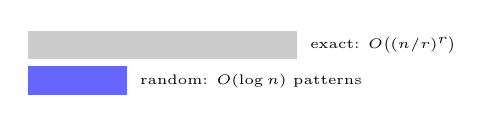
\begin{tikzpicture}[scale=0.9]
        \fill[gray!40] (0,0.5) rectangle (3.8,0.9);
        \node[right, font=\tiny] at (3.85,0.7) {exact: $O\!\left((\nn/\rrank)^{\rrank}\right)$};
        \fill[blue!60] (0,0) rectangle (1.4,0.4);
        \node[right, font=\tiny] at (1.45,0.2) {random: $O(\log\nn)$ patterns};
      \end{tikzpicture}
    \end{column}
    \hfill
    \begin{column}{0.50\textwidth}
      \textbf{Random sampling idea:}
      \vspace{0.2em}
      \begin{center}
      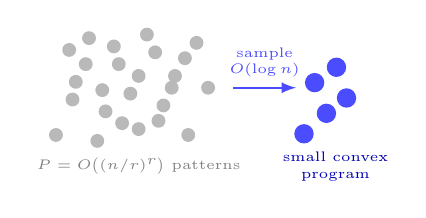
\begin{tikzpicture}[scale=1.0, >=latex]
        % Large cloud of gray dots (P exponentially many patterns)
        \foreach \px/\py in {
            0.00/0.10, 0.12/0.55, 0.25/0.05, 0.08/0.82, 0.20/0.92,
            0.38/0.70, 0.50/0.15, 0.45/0.45, 0.60/0.80, 0.30/0.30,
            0.65/0.35, 0.72/0.60, 0.80/0.10, 0.85/0.88, 0.55/0.95,
            0.10/0.40, 0.40/0.20, 0.70/0.50, 0.18/0.70, 0.78/0.75,
            0.35/0.85, 0.62/0.22, 0.92/0.50, 0.50/0.60, 0.28/0.48} {
          \fill[gray!55] (\px*2.1, \py*1.5) circle (2.5pt);
        }
        \node[font=\tiny, gray, align=center] at (1.05, -0.25)
          {$P = O\!\left((\nn/\rrank)^{\rrank}\right)$ patterns};
        % Arrow
        \draw[->, thick, blue!70] (2.25, 0.75) -- (3.05, 0.75)
          node[midway, above, font=\tiny, align=center]
            {sample\\$O(\log n)$};
        % Selected subset (5 highlighted blue dots)
        \foreach \px/\py in {0.0/0.05, 0.18/0.55, 0.38/0.25, 0.55/0.70, 0.72/0.40} {
          \fill[blue!70] (3.15 + \px*0.75, 0.1 + \py*1.3) circle (3.5pt);
        }
        \node[font=\tiny, blue!70!black, align=center] at (3.55, -0.25)
          {small convex\\program};
      \end{tikzpicture}
      \end{center}
    \end{column}
  \end{columns}

  \vspace{0.5em}

  % --- BOTTOM HALF: approximation guarantee centred ---
  \begin{center}
    \textbf{Approximation guarantee (Thm.\ 2.1):}\quad
    $\Pstar \;\leq\; \ptildestar \;\leq\; \CC\sqrt{\log 2\nn}\;\Pstar$\\[4pt]
    \textit{\footnotesize First poly-time approximation guarantee for regularized ReLU networks.}
  \end{center}

  % SOURCE: Kim & Pilanci 2024, Theorem 2.1 (arxiv-2402.03625, line 128).
\end{frame}


% ---- SLIDE 6b: CRONOS --- FENG, FRANGELLA & PILANCI 2023 ----
\begin{frame}{CRONOS: Scalable GPU Solver --- Feng, Frangella \& Pilanci (2023)}

  \begin{columns}[T]
    \begin{column}{0.50\textwidth}
      \textbf{Adam vs.\ CRONOS-AM on ImageNet:}
      \vspace{0.3em}

      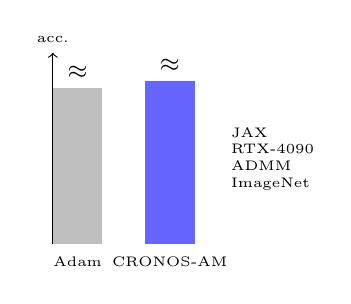
\begin{tikzpicture}[scale=0.9]
        \fill[gray!50]  (0,0) rectangle (0.7,2.2);
        \fill[blue!60]  (1.3,0) rectangle (2.0,2.3);
        \node[below, font=\tiny] at (0.35,-0.05)  {Adam};
        \node[below, font=\tiny] at (1.65,-0.05)  {CRONOS-AM};
        \node[above, font=\tiny] at (0.35,2.2) {\small$\approx$};
        \node[above, font=\tiny] at (1.65,2.3) {\small$\approx$};
        \draw[->] (0,0) -- (0,2.7) node[above, font=\tiny] {acc.};
        \node[font=\tiny, align=left] at (3.1,1.2) {JAX\\ RTX-4090\\ ADMM\\ ImageNet};
      \end{tikzpicture}

      \vspace{0.4em}
      \begin{itemize}\small
        \item Matches/beats tuned Adam
        \item Essentially no hyperparameters
        \item Global opt.\ guarantee (2-layer)
      \end{itemize}
    \end{column}
    \hfill
    \begin{column}{0.47\textwidth}
      \begin{center}
        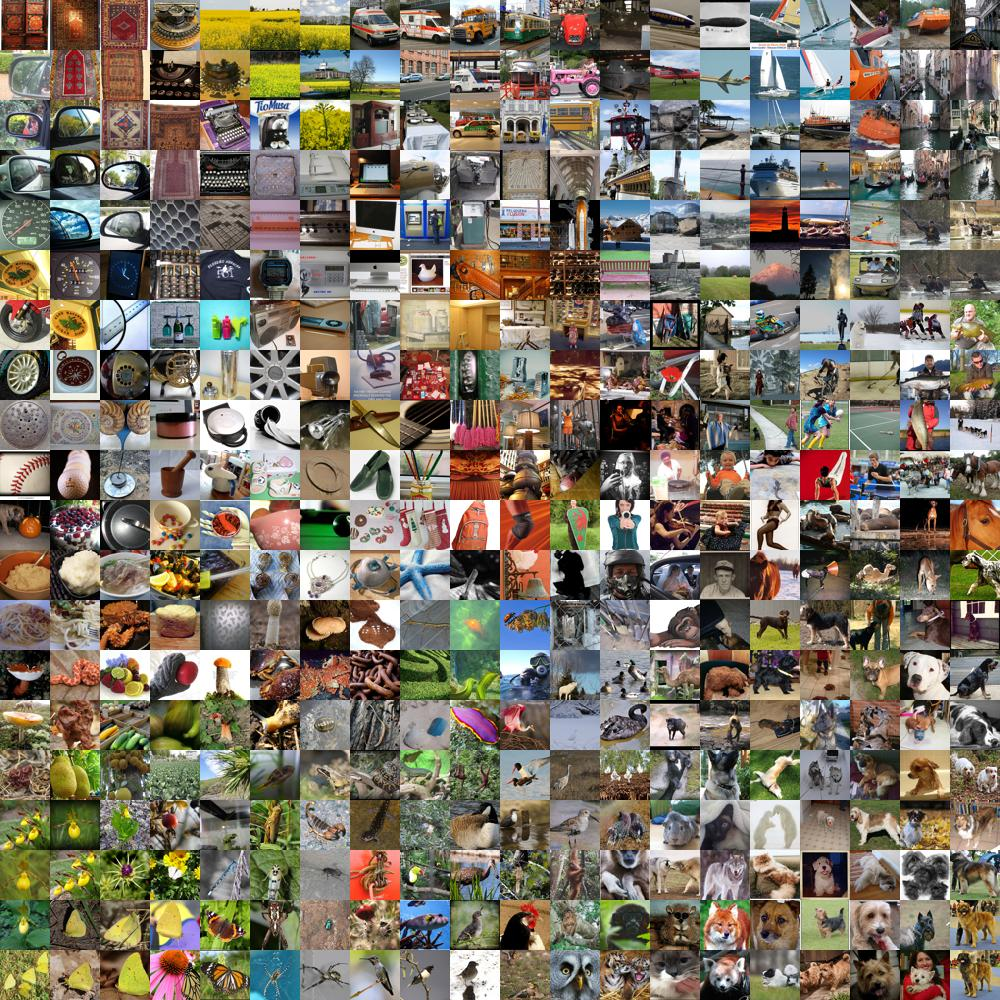
\includegraphics[width=\textwidth,height=0.52\textheight,keepaspectratio]{imagenet-grid.jpg}\\[2pt]
        \tiny ImageNet: 1000 classes, 1.2M training images
      \end{center}
    \end{column}
  \end{columns}

  % SOURCE: Feng, Frangella & Pilanci 2023 (user-8652-CRONOS, lines 26, 40).
\end{frame}


% ============================================================
% ACT 4: CLOSE (target: 0:20, Slide 7)
% ============================================================

% ---- SLIDE 7: TAKEAWAY (7:00-7:20, 20 seconds) ----
% SPEAKING TIME: ~20 seconds (the landing --- must not be cut)
% TIMING CHECK: Talk ends at 8:00. Hand over to Q&A.
%
% SPEAKING NOTES:
% Speak slower than normal. The audience is reading as you speak.
% Use the SHORT spoken version (30 words, ~12 seconds):
%   "ReLU training was secretly convex. Width gives you the bridge,
%    architecture decides whether it holds at depth, and a sqrt(log n)
%    factor makes it tractable in practice."
%
% Walk down the three bullet points while pointing at the three words:
%   "Width, architecture, log n. That is the talk."
% Thank them, stop, hand over.
%
% Do NOT re-raise the open question from Slide 7.
% This slide is the landing, not a new idea.
%
% NO BRIDGE -- THIS IS THE END.
%
\begin{frame}{Takeaway}

  \vspace{0.5em}
  \begin{center}
    \large\textbf{%
      ReLU network training was never really non-convex ---\\[4pt]
      and whether the hidden convex program is exact, tractable,\\
      and practically solvable depends on three things:
    }\\[0.8em]
    \Large\textbf{width \quad|\quad architecture \quad|\quad} {\Large$\bm{\log n}$}
  \end{center}

  \vspace{0.8em}
  \begin{columns}[t]
    \begin{column}{0.3\textwidth}
      \centering
      \textbf{width}\\
      \small Pilanci-Ergen 2020\\
      $\mm \geq \mstar$
    \end{column}
    \begin{column}{0.35\textwidth}
      \centering
      \textbf{architecture}\\
      \small Wang-Ergen-Pilanci 2021\\
      parallel branches
    \end{column}
    \begin{column}{0.3\textwidth}
      \centering
      \textbf{$\bm{\log n}$}\\
      \small Kim-Pilanci 2024\\
      $\sqrt{\log n}$ approximation
    \end{column}
  \end{columns}

  \vspace{0.8em}
  \begin{center}
    \textit{Thank you --- questions welcome.}
  \end{center}
\end{frame}


% ============================================================
% REFERENCES
% ============================================================

\begin{frame}[allowframebreaks]{References}
  \printbibliography[heading=none]
\end{frame}


% ============================================================
% APPENDIX: BACKUP SLIDES (Q&A, after_only format)
% ============================================================

\appendix

% ---- BACKUP B1: GENERALISATION, NOT TRAINING LOSS ----
% TRIGGER: Use if asked "Does the zero-duality-gap result say anything about
%   generalisation, or only training loss?" (QA-B2 -- highest-stakes Q, most
%   likely to be asked; prepare this one cold.)
%
% SPEAKER SCRIPT:
% "Only training loss. The Pilanci-Ergen programme characterises the global
%  optimum of the regularised training objective -- it tells you what the
%  optimal network looks like and how to compute it. It does not on its own
%  give you a bound on test error. There is a natural hope that the polytope
%  structure of the optimal set will eventually feed into a generalisation
%  bound, and there is active work in that direction, but the field has not
%  yet produced a clean theorem of the form 'zero duality gap implies
%  generalisation bound X.' It is a genuine open direction -- arguably the
%  most important one."
%
\begin{frame}{B1: Generalisation, Not Training Loss}
  \begin{columns}[c]
    \begin{column}{0.55\textwidth}
      \begin{itemize}
        \item Zero duality gap $=$ global optimum of \textbf{training loss}
        \item Test error / generalisation bounds: \textbf{NOT} covered
        \item Optimal-set polytope $\to$ hope for future generalisation bounds
        \item The most important honest thing to say about this work
      \end{itemize}
    \end{column}
    \begin{column}{0.42\textwidth}
      % FIGURE DESCRIPTION: Two boxes connected by an arrow.
      % Left: "training loss -- characterised by the convex reformulation."
      % Right: "test error -- no theorem yet."
      % Arrow label: "active research direction?"
      \begin{center}
        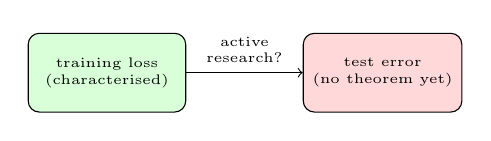
\begin{tikzpicture}
          \node[draw, fill=green!15, rounded corners, font=\tiny, align=center,
                minimum width=2cm, minimum height=1cm] (train) at (0,0)
            {training loss\\(characterised)};
          \node[draw, fill=red!15, rounded corners, font=\tiny, align=center,
                minimum width=2cm, minimum height=1cm] (test) at (3.5,0)
            {test error\\(no theorem yet)};
          \draw[->] (train)--(test)
            node[midway, above, font=\tiny, align=center]
              {active\\research?};
        \end{tikzpicture}
      \end{center}
    \end{column}
  \end{columns}
  % SOURCE: analysis/open-questions.md QA-B2
\end{frame}


% ---- BACKUP B2: DOES THIS EXTEND TO TRANSFORMERS? ----
% TRIGGER: Use if asked "Does this extend to transformers?"
%   (QA-B3 -- second-most-likely Q&A question.)
%
% SPEAKER SCRIPT:
% "Not in a published global-optimality sense. The whole convex-reformulation
%  machinery depends structurally on ReLU being piecewise linear, which is
%  what lets you enumerate hyperplane arrangement patterns. Attention is
%  softmax, which is smooth -- not piecewise linear -- and that structural
%  property does not carry over. Kim and Pilanci explicitly flag transformers
%  as something they want to extend to -- that honest flag is itself the
%  answer. It is probably the biggest single open direction in this area."
%
\begin{frame}{B2: Does This Extend to Transformers?}
  \begin{columns}[c]
    \begin{column}{0.52\textwidth}
      \begin{itemize}
        \item Convex reformulation requires ReLU: piecewise linear
        \item Attention (softmax) is smooth --- no hyperplane patterns
        \item Extension to transformers: \textbf{explicitly open}\\
              (\citeauthor{arxiv2402.03625}, \citeyear{arxiv2402.03625} conclusion)
        \item Polynomial activations: partial via SDP\\
              (\citeauthor{arxiv2101.02429}, \citeyear{arxiv2101.02429})
      \end{itemize}
    \end{column}
    \begin{column}{0.44\textwidth}
      % FIGURE DESCRIPTION: Three boxes in a row:
      % "ReLU (piecewise linear)" -- green checkmark
      % "Attention / softmax (smooth)" -- red X
      % "Polynomial activations (SDP lifts)" -- yellow tilde
      \begin{center}
        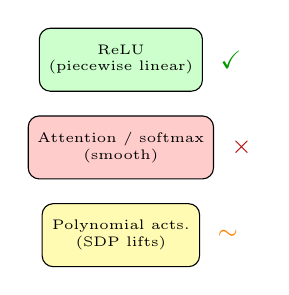
\begin{tikzpicture}[node distance=0.4cm]
          \node[draw, fill=green!20, rounded corners, font=\tiny, align=center,
                minimum width=2cm, minimum height=0.8cm] (relu)
            {ReLU\\(piecewise linear)};
          \node[font=\small, right=0.1cm of relu, green!60!black] {$\checkmark$};
          \node[draw, fill=red!20, rounded corners, font=\tiny, align=center,
                minimum width=2cm, minimum height=0.8cm, below=0.3cm of relu] (att)
            {Attention / softmax\\(smooth)};
          \node[font=\small, right=0.1cm of att, red!70!black] {$\times$};
          \node[draw, fill=yellow!30, rounded corners, font=\tiny, align=center,
                minimum width=2cm, minimum height=0.8cm, below=0.3cm of att] (poly)
            {Polynomial acts.\\(SDP lifts)};
          \node[font=\small, right=0.1cm of poly, orange] {$\sim$};
        \end{tikzpicture}
      \end{center}
    \end{column}
  \end{columns}
  % SOURCE: Kim & Pilanci 2024 (arxiv-2402.03625, line 461); QA-B3
\end{frame}


% ---- BACKUP B3: RELATIONSHIP TO NTK ----
% TRIGGER: Use if asked "How does the convex reformulation relate to the Neural
%   Tangent Kernel? Isn't NTK already the 'convex' story for neural networks?"
%   (QA-A1)
%
% SPEAKER SCRIPT:
% "NTK is a strict special case of the convex reformulation -- this is the
%  result of Dwaraknath, Ergen, and Pilanci in 2023. The convex reformulation
%  of a gated ReLU network is an instance of Multiple Kernel Learning, and
%  the NTK is what you get when the mask weights are target-independent --
%  the 'lazy' regime where no feature learning happens. Iteratively reweighting
%  the MKL kernel recovers the full convex optimum, and the difference between
%  the NTK and the full convex solution is exactly what we call feature learning.
%  The two views are not in conflict; the convex view contains NTK."
%
\begin{frame}{B3: Relationship to NTK}
  \begin{columns}[c]
    \begin{column}{0.52\textwidth}
      \begin{itemize}
        \item NTK (Jacot 2018): infinite width, no feature learning
        \item Convex reformulation: exact at finite width, with feature learning
        \item \citeauthor{arxiv2309.15096} (\citeyear{arxiv2309.15096}):\\
              NTK is a special case of the MKL structure
        \item Iterative reweighting upgrades NTK to the full convex solution
        \item feature learning $=$ the gap between NTK and full convex solution
      \end{itemize}
    \end{column}
    \begin{column}{0.44\textwidth}
      % FIGURE DESCRIPTION: Nested circles (Venn).
      % Small inner: "NTK -- lazy regime, target-independent mask weights."
      % Large outer: "Convex reformulation -- MKL, target-dependent."
      % Arrow: "iterative reweighting." Caption: "feature learning = the gap."
      \begin{center}
        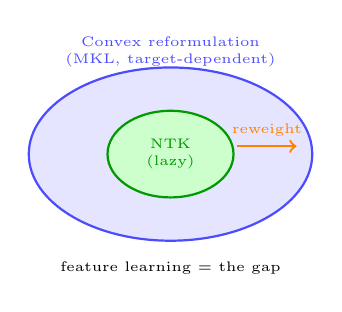
\begin{tikzpicture}
          \fill[blue!10] (0,0) ellipse (1.8cm and 1.1cm);
          \draw[thick, blue!70] (0,0) ellipse (1.8cm and 1.1cm);
          \node[font=\tiny, blue!70, align=center] at (0, 1.3)
            {Convex reformulation\\ (MKL, target-dependent)};
          \fill[green!20] (0,0) ellipse (0.8cm and 0.55cm);
          \draw[thick, green!60!black] (0,0) ellipse (0.8cm and 0.55cm);
          \node[font=\tiny, green!60!black, align=center] at (0,0)
            {NTK\\ (lazy)};
          \draw[->, thick, orange] (0.85,0.1) -- (1.6,0.1)
            node[above, font=\tiny, midway] {reweight};
          \node[font=\tiny, align=center] at (0,-1.45)
            {feature learning $=$ the gap};
        \end{tikzpicture}
      \end{center}
    \end{column}
  \end{columns}
  % SOURCE: Dwaraknath, Ergen & Pilanci 2023 (arxiv-2309.15096); QA-A1
\end{frame}


% ---- BACKUP B4: WHAT ABOUT RESNETS? ----
% TRIGGER: Use if asked "What about ResNets? Do skip connections fit into this
%   framework?" (QA-A3)
%
% SPEAKER SCRIPT:
% "Yes, cleanly. Wang, Ergen, and Pilanci show that a ResNet with weight decay
%  fits the parallel-network framework as a special case -- a residual block is
%  structurally a two-branch parallel network, with one branch being the identity.
%  This is actually part of why the paper interprets modern architectures like
%  ResNeXt, Inception, and SqueezeNet as empirically successful: they were already
%  built in a parallel pattern, and that parallel pattern is what restores strong
%  duality at depth beyond two."
%
\begin{frame}{B4: What About ResNets?}
  \begin{columns}[c]
    \begin{column}{0.52\textwidth}
      \begin{itemize}
        \item ResNet residual block $=$ 2-branch parallel network
        \item Branch 1: \textbf{identity} path
        \item Branch 2: \textbf{transform} path (Conv $\to$ BN $\to$ ReLU)
        \item \citeauthor{arxiv2110.06482} (\citeyear{arxiv2110.06482}):\\
              ResNets $+$ weight decay $\subseteq$ parallel-network framework
        \item Strong duality restored: inherits zero-duality-gap result
      \end{itemize}
    \end{column}
    \begin{column}{0.44\textwidth}
      % FIGURE DESCRIPTION: Residual block redrawn as 2-branch parallel network.
      % Branch 1: identity path (x -> output). Branch 2: Conv->BN->ReLU.
      % Outputs summed. Label: "a ResNet block *is* a parallel network."
      \begin{center}
        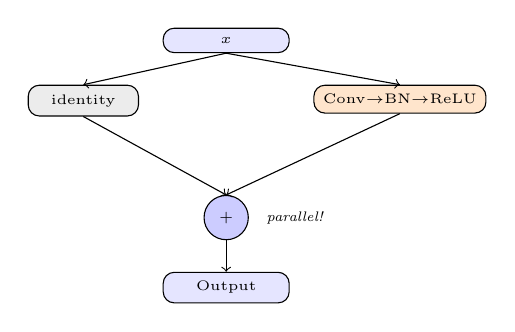
\begin{tikzpicture}[node distance=0.5cm, font=\tiny]
          \node[draw, rounded corners, fill=blue!10, minimum width=1.6cm] (inp) {$x$};
          % Branch 1: identity
          \node[draw, rounded corners, fill=gray!15, minimum width=1.4cm,
                below left=0.4cm and 0.3cm of inp] (id) {identity};
          % Branch 2: transform
          \node[draw, rounded corners, fill=orange!20, minimum width=1.4cm,
                below right=0.4cm and 0.3cm of inp] (tr) {Conv$\to$BN$\to$ReLU};
          % Sum
          \node[draw, circle, fill=blue!20, below=1.8cm of inp] (sum) {$+$};
          \node[draw, rounded corners, fill=blue!10, minimum width=1.6cm,
                below=0.4cm of sum] (out) {Output};
          \draw[->] (inp.south) -- (id.north);
          \draw[->] (inp.south) -- (tr.north);
          \draw[->] (id.south) -- (sum.north);
          \draw[->] (tr.south) -- (sum.north);
          \draw[->] (sum) -- (out);
          \node[font=\tiny, right=0.1cm of sum] {\textit{parallel!}};
        \end{tikzpicture}
      \end{center}
    \end{column}
  \end{columns}
  % SOURCE: Wang, Ergen & Pilanci 2021 (arxiv-2110.06482); QA-A3
\end{frame}


% ============================================================
% END OF DOCUMENT
% ============================================================
\end{document}
